\section{Image Data: Intel Image Classification}
\label{sec:image}

\subsection{Task Objective and Dataset}

This task classifies a natural scene image into one of six labels: \textit{buildings}, \textit{forest}, \textit{glacier}, \textit{mountain}, \textit{sea}, and \textit{street}. The selected source is the Intel Image Classification dataset on Kaggle \cite{intel}. It contains 17,034 labelled RGB JPEG images. Every original image is 150 by 150 pixels, which is above the course recommendation of a short side of 128 pixels. The dataset has 14,034 images in its source training folder and 3,000 images in a separate source test folder.

The image labels are supplied by the dataset. This project does not claim to discover a new scene category or to judge whether a source label is perfect. Its purpose is to build a clear and reproducible classroom classifier: inspect the images, define a fair split, compare two understandable pretrained approaches, and then measure the selected approach on images that were not used earlier.

\begin{importantbox}
\textbf{Task fit.} The dataset has more than 5,000 images and more than three target classes. It is therefore large enough for the Image-data task, while the six everyday scene classes remain understandable for a first image-classification project.
\end{importantbox}

\subsection{Dataset Structure and Image EDA}

The downloaded dataset has two labelled folders: \texttt{seg\_train} and \texttt{seg\_test}. Each class has its own subfolder, so the parent folder name becomes the target label. The notebook uses \texttt{torchvision.datasets.ImageFolder} to read this simple structure. It does not read a hidden metadata column or a filename-derived target. The class order is alphabetical and is fixed as buildings, forest, glacier, mountain, sea, and street.

Table~\ref{tab:intel-class-counts} shows the source distribution. The class counts are similar but not identical. Glacier has the most source-test images (553), while buildings has the fewest (437). For this reason, ordinary accuracy is reported together with balanced accuracy and macro F1. Macro F1 first computes an F1 score for each class and then gives every class the same weight. This makes a model that only succeeds on a common class less attractive.

\begin{table}[H]
\centering
\caption{Intel Image Classification source folders and labels.}
\label{tab:intel-class-counts}
\begin{tabular}{lrrr}
\toprule
\textbf{Scene class} & \textbf{Source train} & \textbf{Source test} & \textbf{Total} \\
\midrule
Buildings & 2,191 & 437 & 2,628 \\
Forest & 2,271 & 474 & 2,745 \\
Glacier & 2,404 & 553 & 2,957 \\
Mountain & 2,512 & 525 & 3,037 \\
Sea & 2,274 & 510 & 2,784 \\
Street & 2,382 & 501 & 2,883 \\
\midrule
\textbf{Total} & \textbf{14,034} & \textbf{3,000} & \textbf{17,034} \\
\bottomrule
\end{tabular}
\end{table}

Figure~\ref{fig:intel-examples} gives one real image from each label. The examples already explain why this is a useful task: forest is visually distinctive because of repeated green texture, while glacier and mountain can share rocks, snow, and sky. Buildings and street can also share urban structures. These overlaps should appear again in the error analysis rather than being hidden behind a single score.

\begin{figure}[H]
\centering
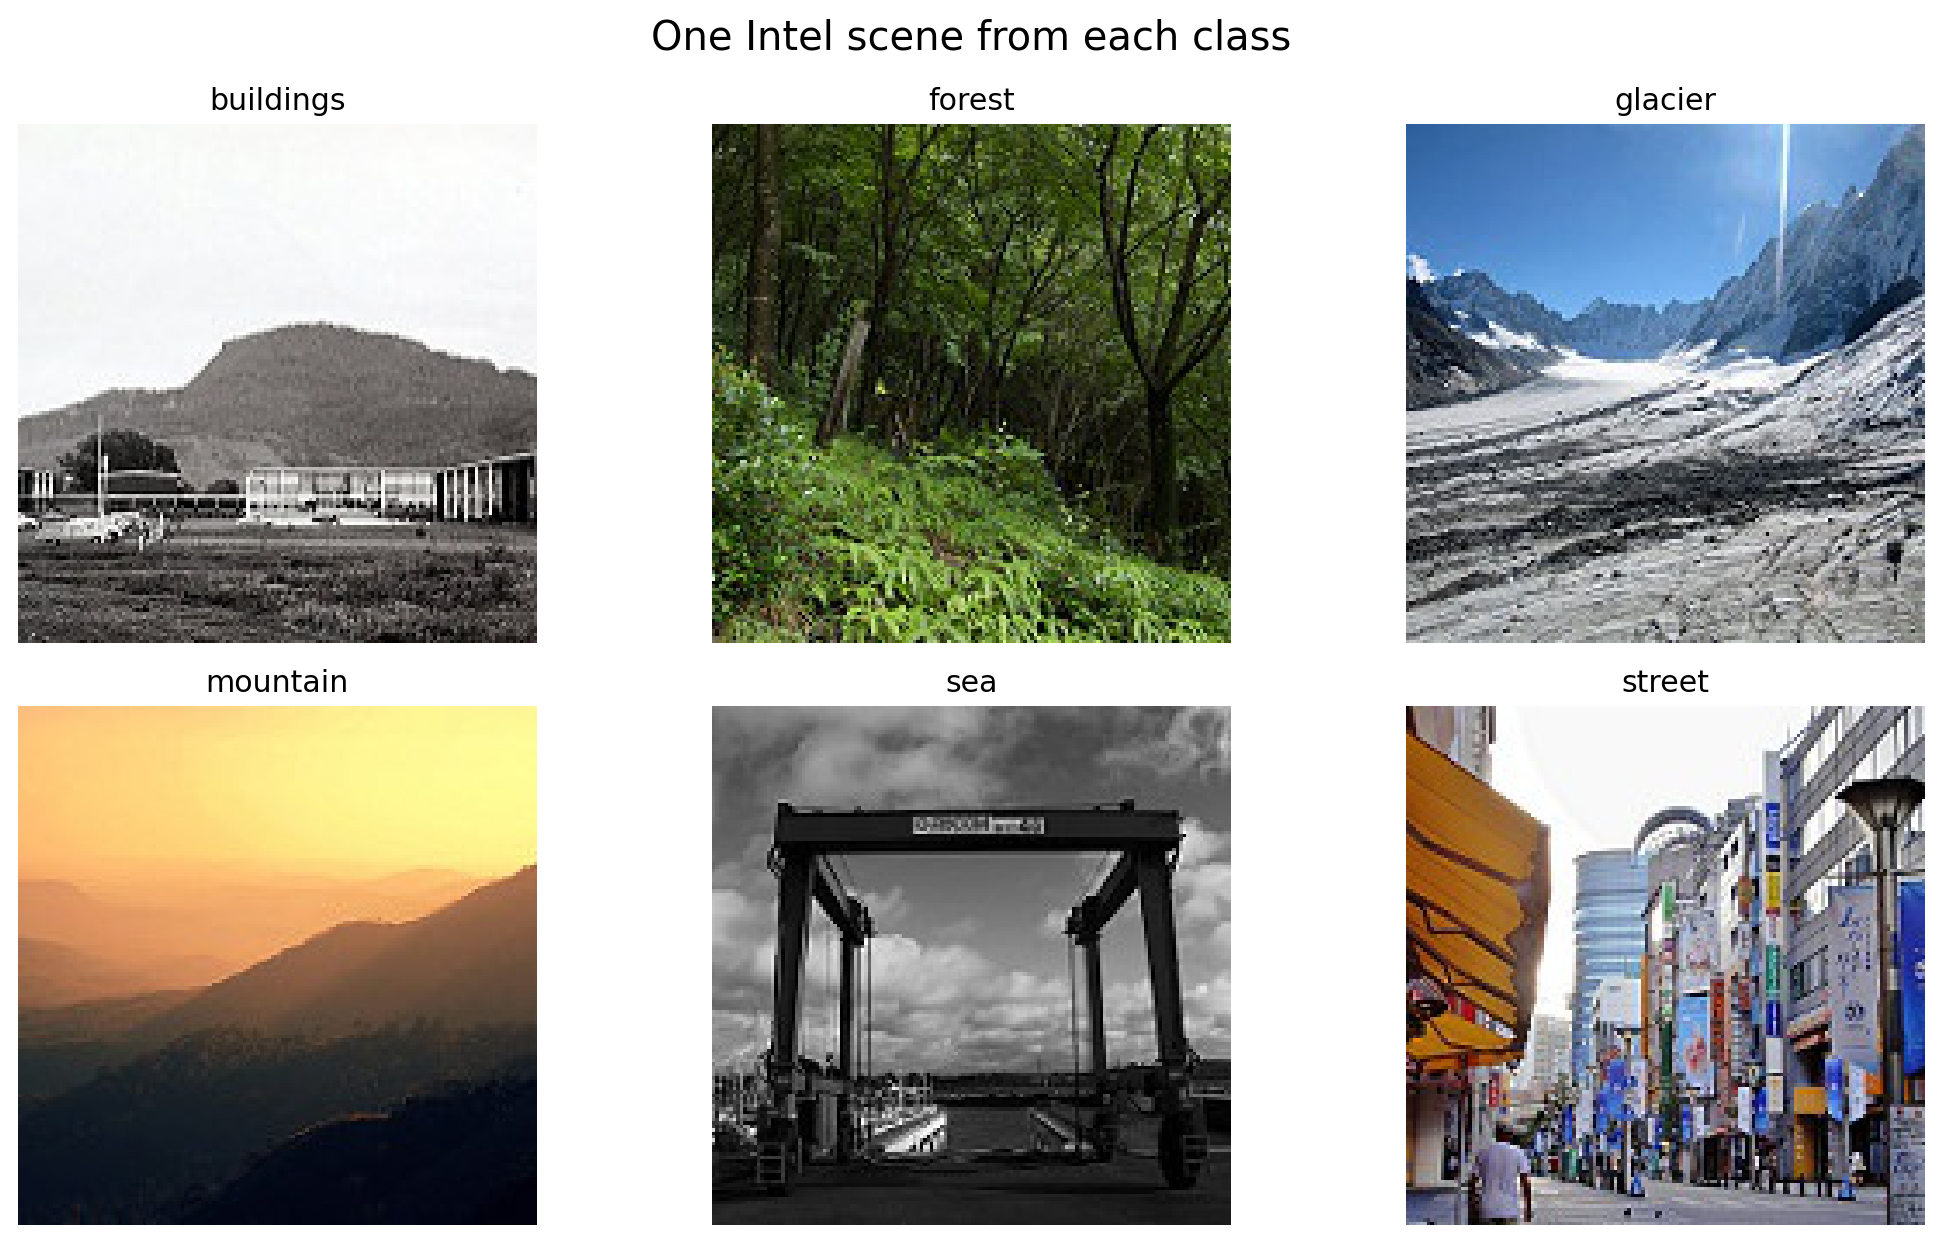
\includegraphics[width=\textwidth]{images/intel_01_scene_examples.png}
\caption{One source image from each Intel scene class.}
\label{fig:intel-examples}
\end{figure}

Figure~\ref{fig:intel-eda} contains two independent EDA plots. The first confirms the per-class counts. The second uses mean pixel brightness as a small quality check. Brightness is not added as a separate model feature. It is only used to show that lighting, snow, clouds, and shadows vary across images, so a consistent image normalization step is necessary before using ImageNet-pretrained weights.

\begin{figure}[H]
\centering
\begin{minipage}{0.52\textwidth}
\centering
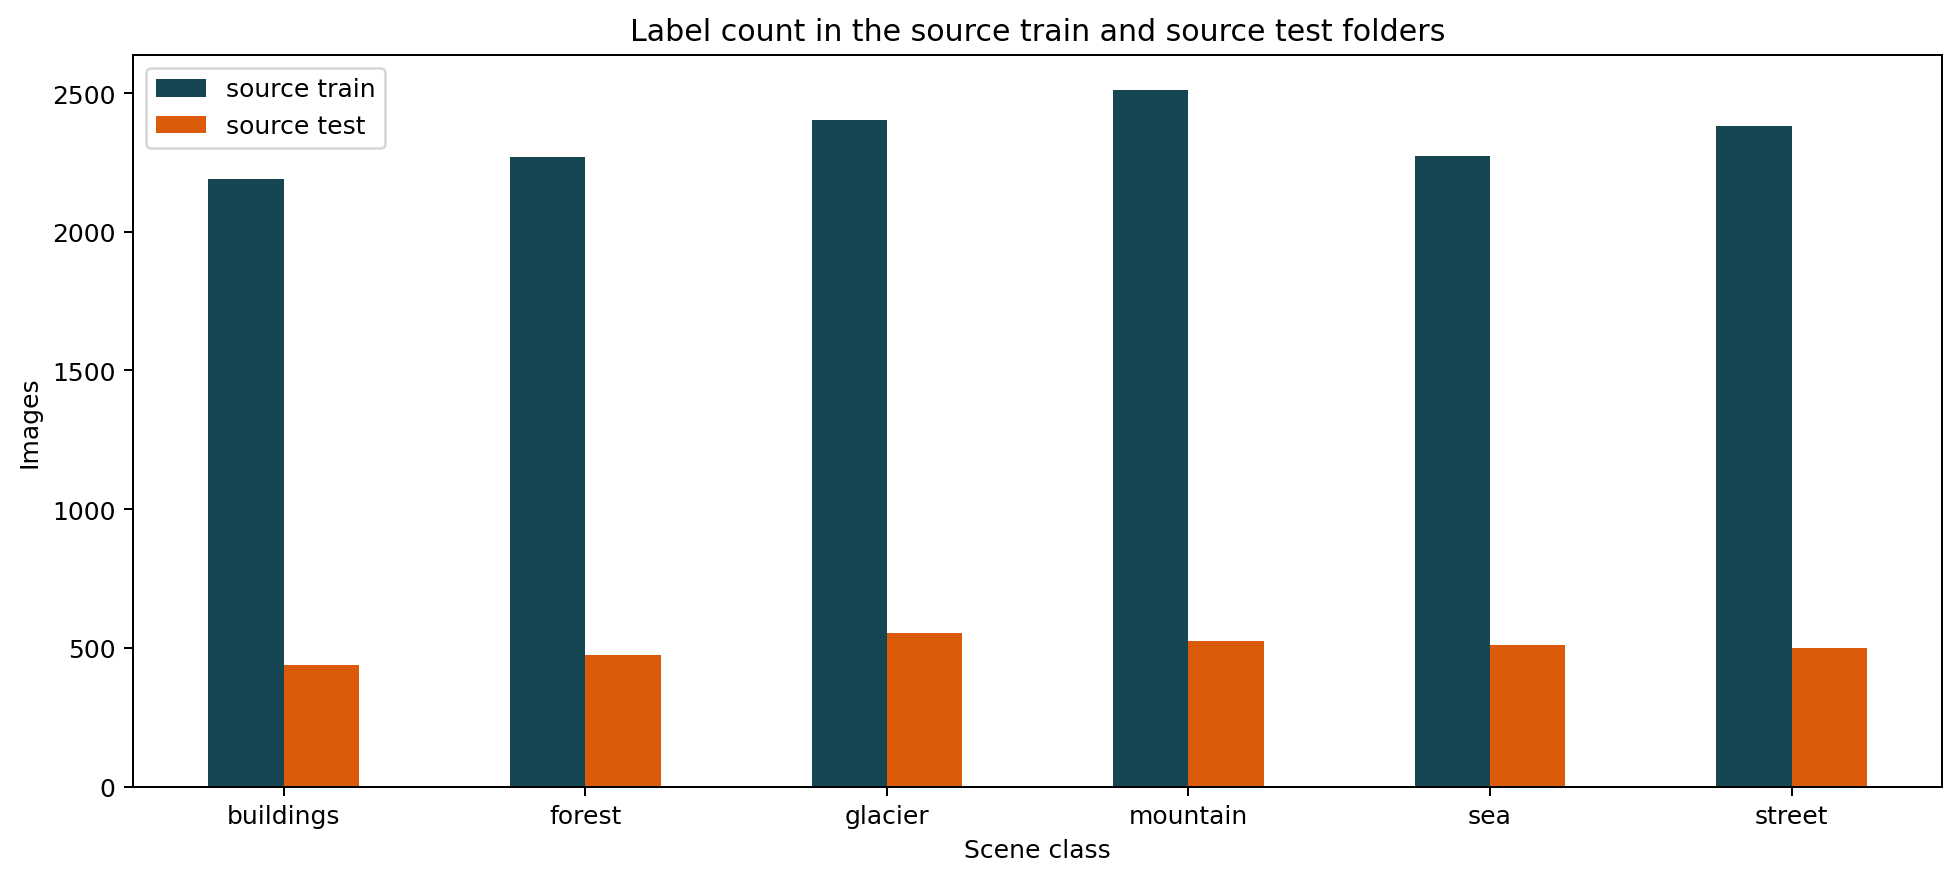
\includegraphics[width=\textwidth]{images/intel_02_class_distribution.png}\\
\small (a) Source class counts
\end{minipage}\hfill
\begin{minipage}{0.42\textwidth}
\centering
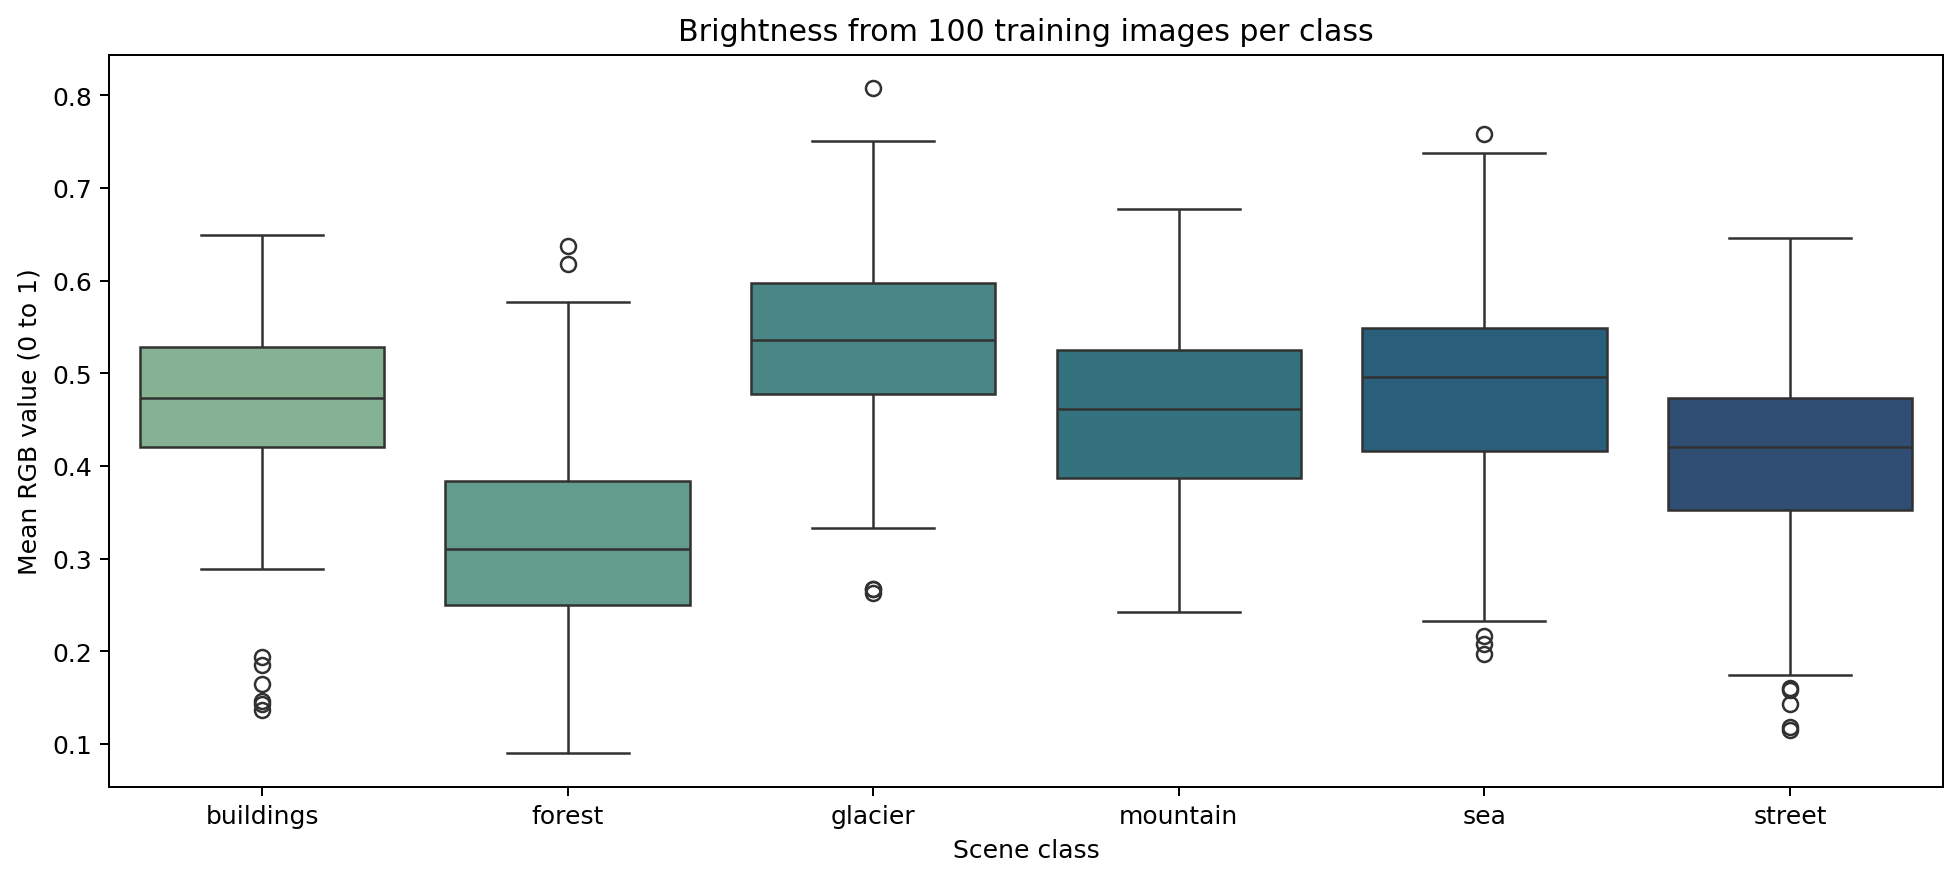
\includegraphics[width=\textwidth]{images/intel_03_brightness_by_class.png}\\
\small (b) Brightness check by class
\end{minipage}
\caption{Simple image EDA. The brightness plot is an inspection result, not an input column.}
\label{fig:intel-eda}
\end{figure}

\subsection{Split, Quality Control, and Leakage Prevention}

The source \texttt{seg\_test} folder is reserved as the final test set from the beginning. It is never used to fit a model, choose an epoch, choose a transform, or compare the two approaches. The source \texttt{seg\_train} folder is split with seed 42 and stratification: 80\% becomes the fitting set and 20\% becomes the validation set. Stratification keeps the six class proportions close to the original source distribution.

\begin{table}[H]
\centering
\caption{Fair split used for the Intel image task.}
\label{tab:intel-split}
\begin{tabular}{lrl}
\toprule
\textbf{Split} & \textbf{Images} & \textbf{Use} \\
\midrule
Training & 11,227 & Fit the Logistic Regression classifier and MobileNetV3 head \\
Validation & 2,807 & Select the final approach using macro F1 \\
Source test & 3,000 & Evaluate the selected approach once at the end \\
\bottomrule
\end{tabular}
\end{table}

The code keeps the source folders separate and uses each image path in only one of these three roles. There is no outcome-like metadata or identifier used as an input: the input is only the RGB image. All 17,034 JPEG files loaded successfully during the executed run. This does not prove that a public dataset has no visually similar pictures, but it prevents the direct leakage that would occur if the provided test folder entered the split or model-selection step.

\subsection{Preprocessing and Augmentation}

MobileNetV3-Small is pretrained on ImageNet. For feature extraction and evaluation, the notebook applies the preprocessing supplied with the pretrained weights: resize, centre crop, tensor conversion, and ImageNet channel normalization. The original data are 150 by 150 pixels; the network receives its standard 224 by 224 view after resizing. This makes the numerical pixel range compatible with the pretrained network.

The training view also uses one simple augmentation: a random horizontal flip. Mirroring a forest, a mountain, or a street does not change its scene label, but it prevents the new classifier head from relying too strongly on a left-right layout. Validation and test images never receive the random flip, so their predictions are repeatable. Figure~\ref{fig:intel-preparation} shows one augmentation example and the five-epoch learning curve.

\begin{figure}[H]
\centering
\begin{minipage}{0.42\textwidth}
\centering
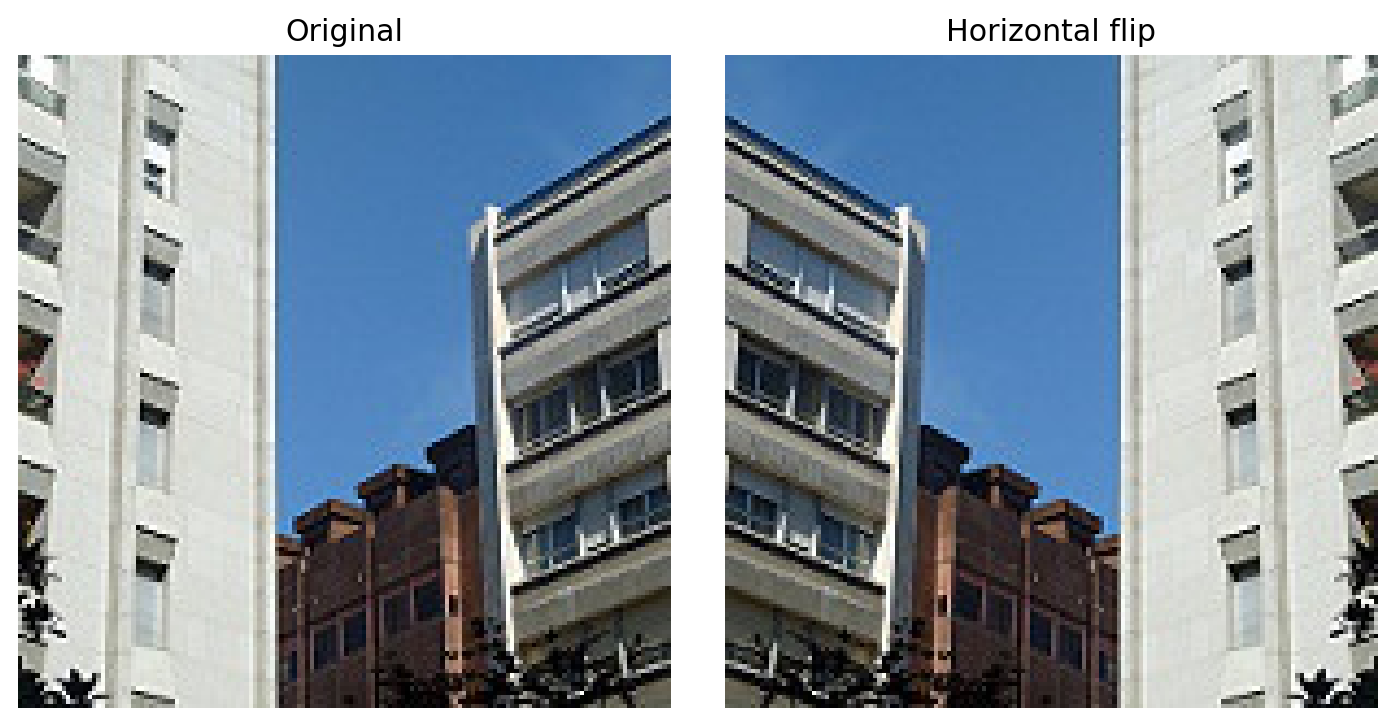
\includegraphics[width=\textwidth]{images/intel_04_augmentation_example.png}\\
\small (a) Random horizontal flip
\end{minipage}\hfill
\begin{minipage}{0.53\textwidth}
\centering
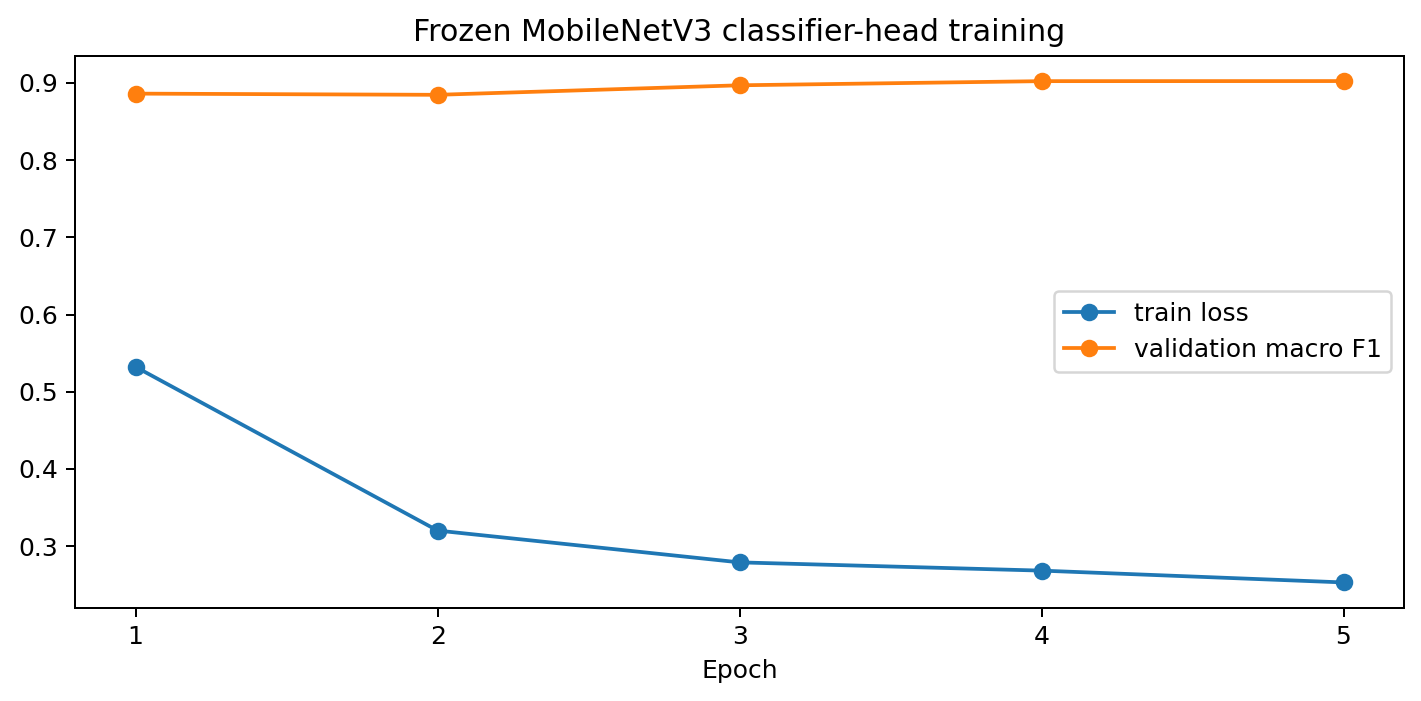
\includegraphics[width=\textwidth]{images/intel_05_training_history.png}\\
\small (b) Frozen-head training history
\end{minipage}
\caption{The only random augmentation and the five-epoch training history.}
\label{fig:intel-preparation}
\end{figure}

\subsection{Model Comparison}

Both candidate models reuse the same pretrained MobileNetV3-Small visual backbone. This meets the deep-learning requirement without asking a beginner to train a convolutional network from scratch. The first model removes the final classifier, so each image becomes a 576-value pretrained feature vector. A balanced Logistic Regression model is then fitted to these vectors. This is a useful simple baseline: the deep network describes visual patterns, and a linear classifier makes the final class decision.

The second model freezes the MobileNetV3 feature layers and replaces its final output layer with a six-class classifier. Only the classifier head is updated for five epochs with Adam, learning rate 0.0003, and class-weighted cross-entropy. This is light transfer learning. It allows the final layer to adapt to the six Intel labels without changing the large pretrained feature extractor.

Table~\ref{tab:intel-validation} compares the models only on validation images. The pretrained-feature Logistic Regression model has the higher validation macro F1 (0.906 versus 0.902), so it is selected before the source-test labels are evaluated. The difference is small, but the selection rule is explicit and does not use the test score.

\begin{table}[H]
\centering
\caption{Validation comparison. Selection is based on macro F1.}
\label{tab:intel-validation}
\begin{tabular}{lrrr}
\toprule
\textbf{Model} & \textbf{Accuracy} & \textbf{Balanced acc.} & \textbf{Macro F1} \\
\midrule
Pretrained features + Logistic Regression & \textbf{0.904} & \textbf{0.906} & \textbf{0.906} \\
Frozen MobileNetV3 head & 0.900 & 0.902 & 0.902 \\
\bottomrule
\end{tabular}
\end{table}

\begin{figure}[H]
\centering
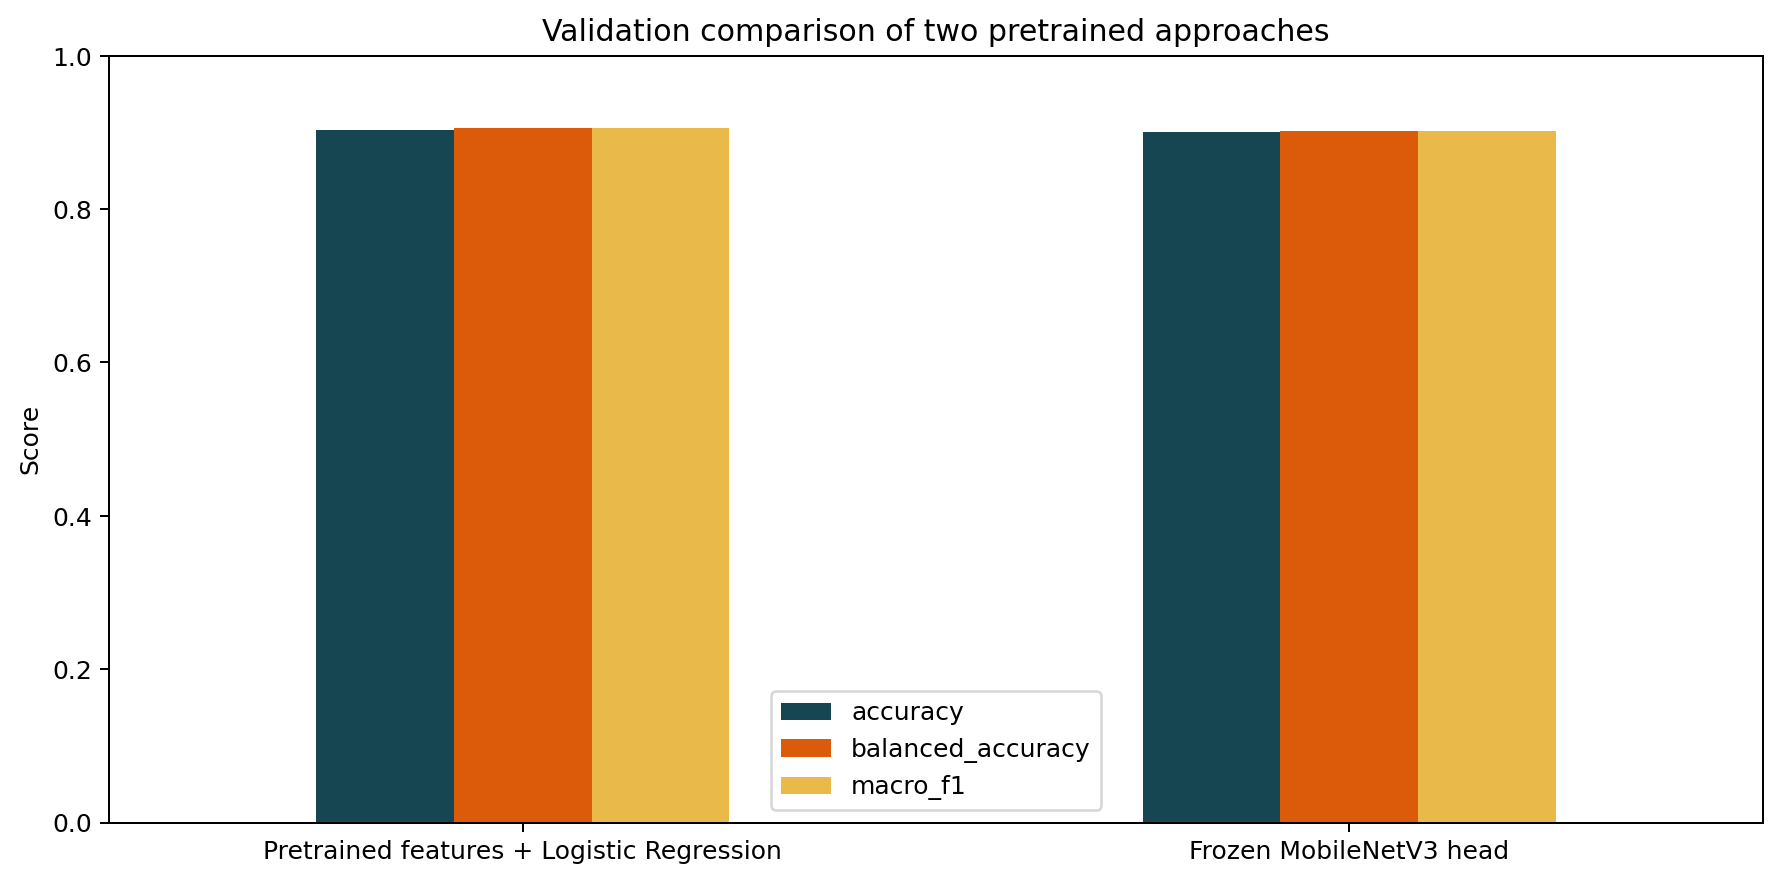
\includegraphics[width=0.80\textwidth]{images/intel_06_model_comparison.png}
\caption{Validation scores for the two pretrained approaches.}
\label{fig:intel-models}
\end{figure}

\subsection{Final Test Evaluation and Error Review}

The selected pretrained-feature Logistic Regression model is evaluated once on the untouched source test folder. It obtains accuracy 0.914, balanced accuracy 0.916, and macro F1 0.916. The close values show that the result is not caused only by one large class. Forest is the easiest class (F1 0.994), while glacier and mountain are harder (F1 0.860 and 0.863). This matches the visual overlap seen in the example images.

\begin{table}[H]
\centering
\caption{Per-class result of the selected model on the 3,000-image source test set.}
\label{tab:intel-test}
\begin{tabular}{lrrr}
\toprule
\textbf{Class} & \textbf{Precision} & \textbf{Recall} & \textbf{F1} \\
\midrule
Buildings & 0.903 & 0.920 & 0.912 \\
Forest & 0.996 & 0.992 & 0.994 \\
Glacier & 0.863 & 0.857 & 0.860 \\
Mountain & 0.867 & 0.859 & 0.863 \\
Sea & 0.938 & 0.949 & 0.943 \\
Street & 0.928 & 0.922 & 0.925 \\
\midrule
\textbf{Macro average} & \textbf{0.916} & \textbf{0.916} & \textbf{0.916} \\
\bottomrule
\end{tabular}
\end{table}

Figure~\ref{fig:intel-confusion} is normalized row by row. A diagonal cell is the recall for one true class. The darker diagonal cells confirm good recognition of forest and sea. The main visible confusion is between glacier and mountain, which is expected because both can contain rock, snow, cloud, and a distant horizon.

\begin{figure}[H]
\centering
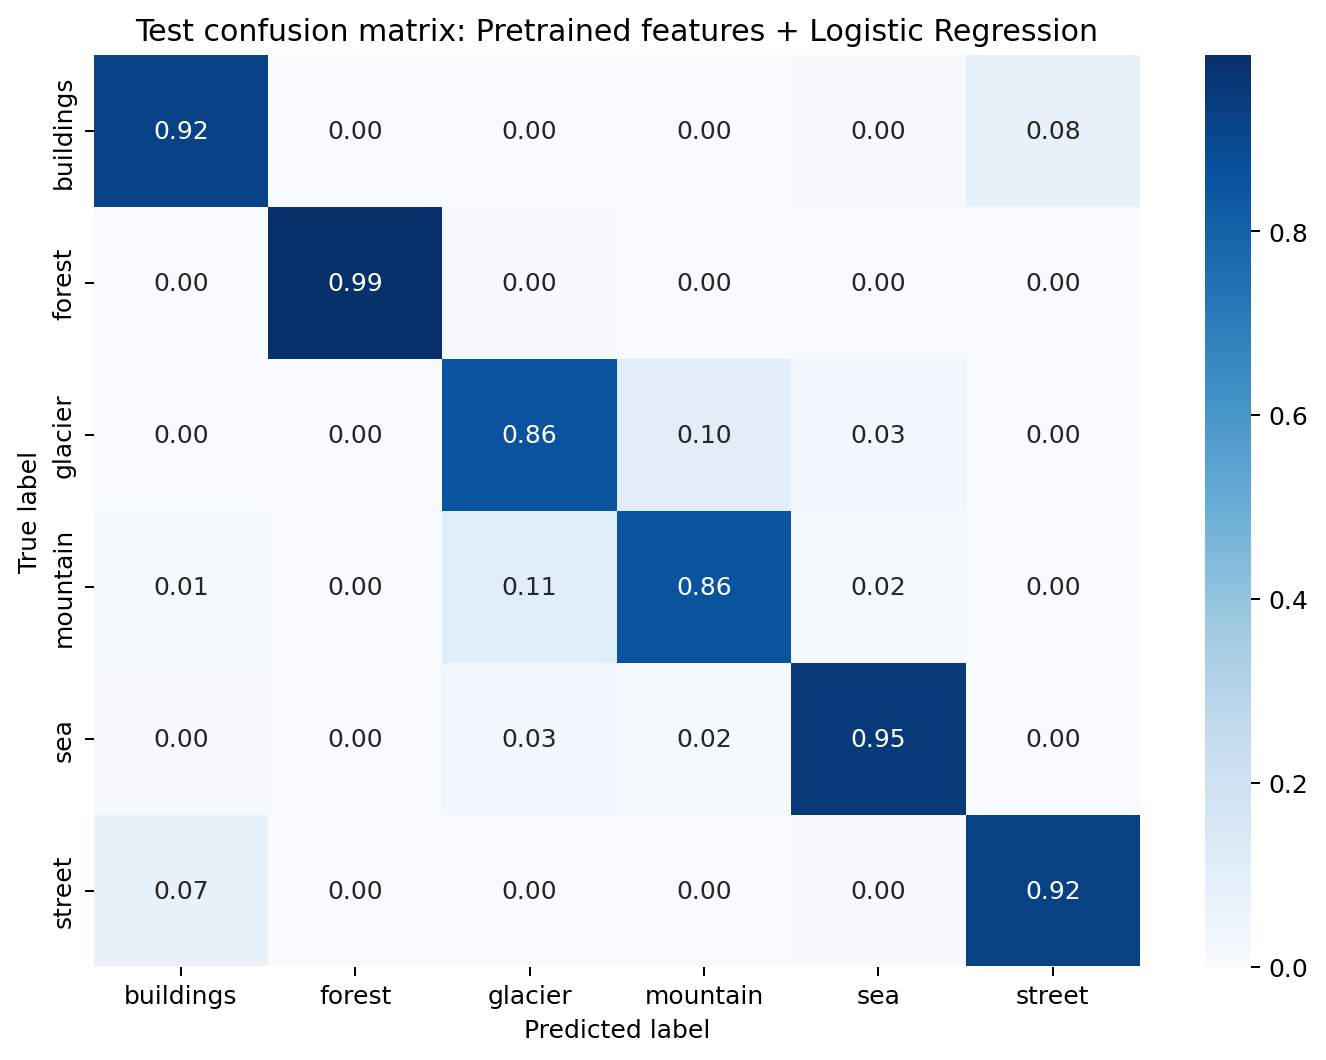
\includegraphics[width=0.90\textwidth]{images/intel_07_confusion_matrix.png}
\caption{Normalized source-test confusion matrix for the selected model.}
\label{fig:intel-confusion}
\end{figure}

There are 257 wrong predictions among the 3,000 test images. The two most frequent directional errors are glacier predicted as mountain (58 images) and mountain predicted as glacier (58 images). Street predicted as buildings (35 images) and buildings predicted as street (33 images) are the next important pair. Figure~\ref{fig:intel-errors} shows twelve concrete mistakes. These examples are more useful than claiming that a 0.916 macro F1 is perfect: scene boundaries can be visually ambiguous, and a model can fail on unusual lighting, distant objects, or mixed scenery.

\begin{figure}[H]
\centering
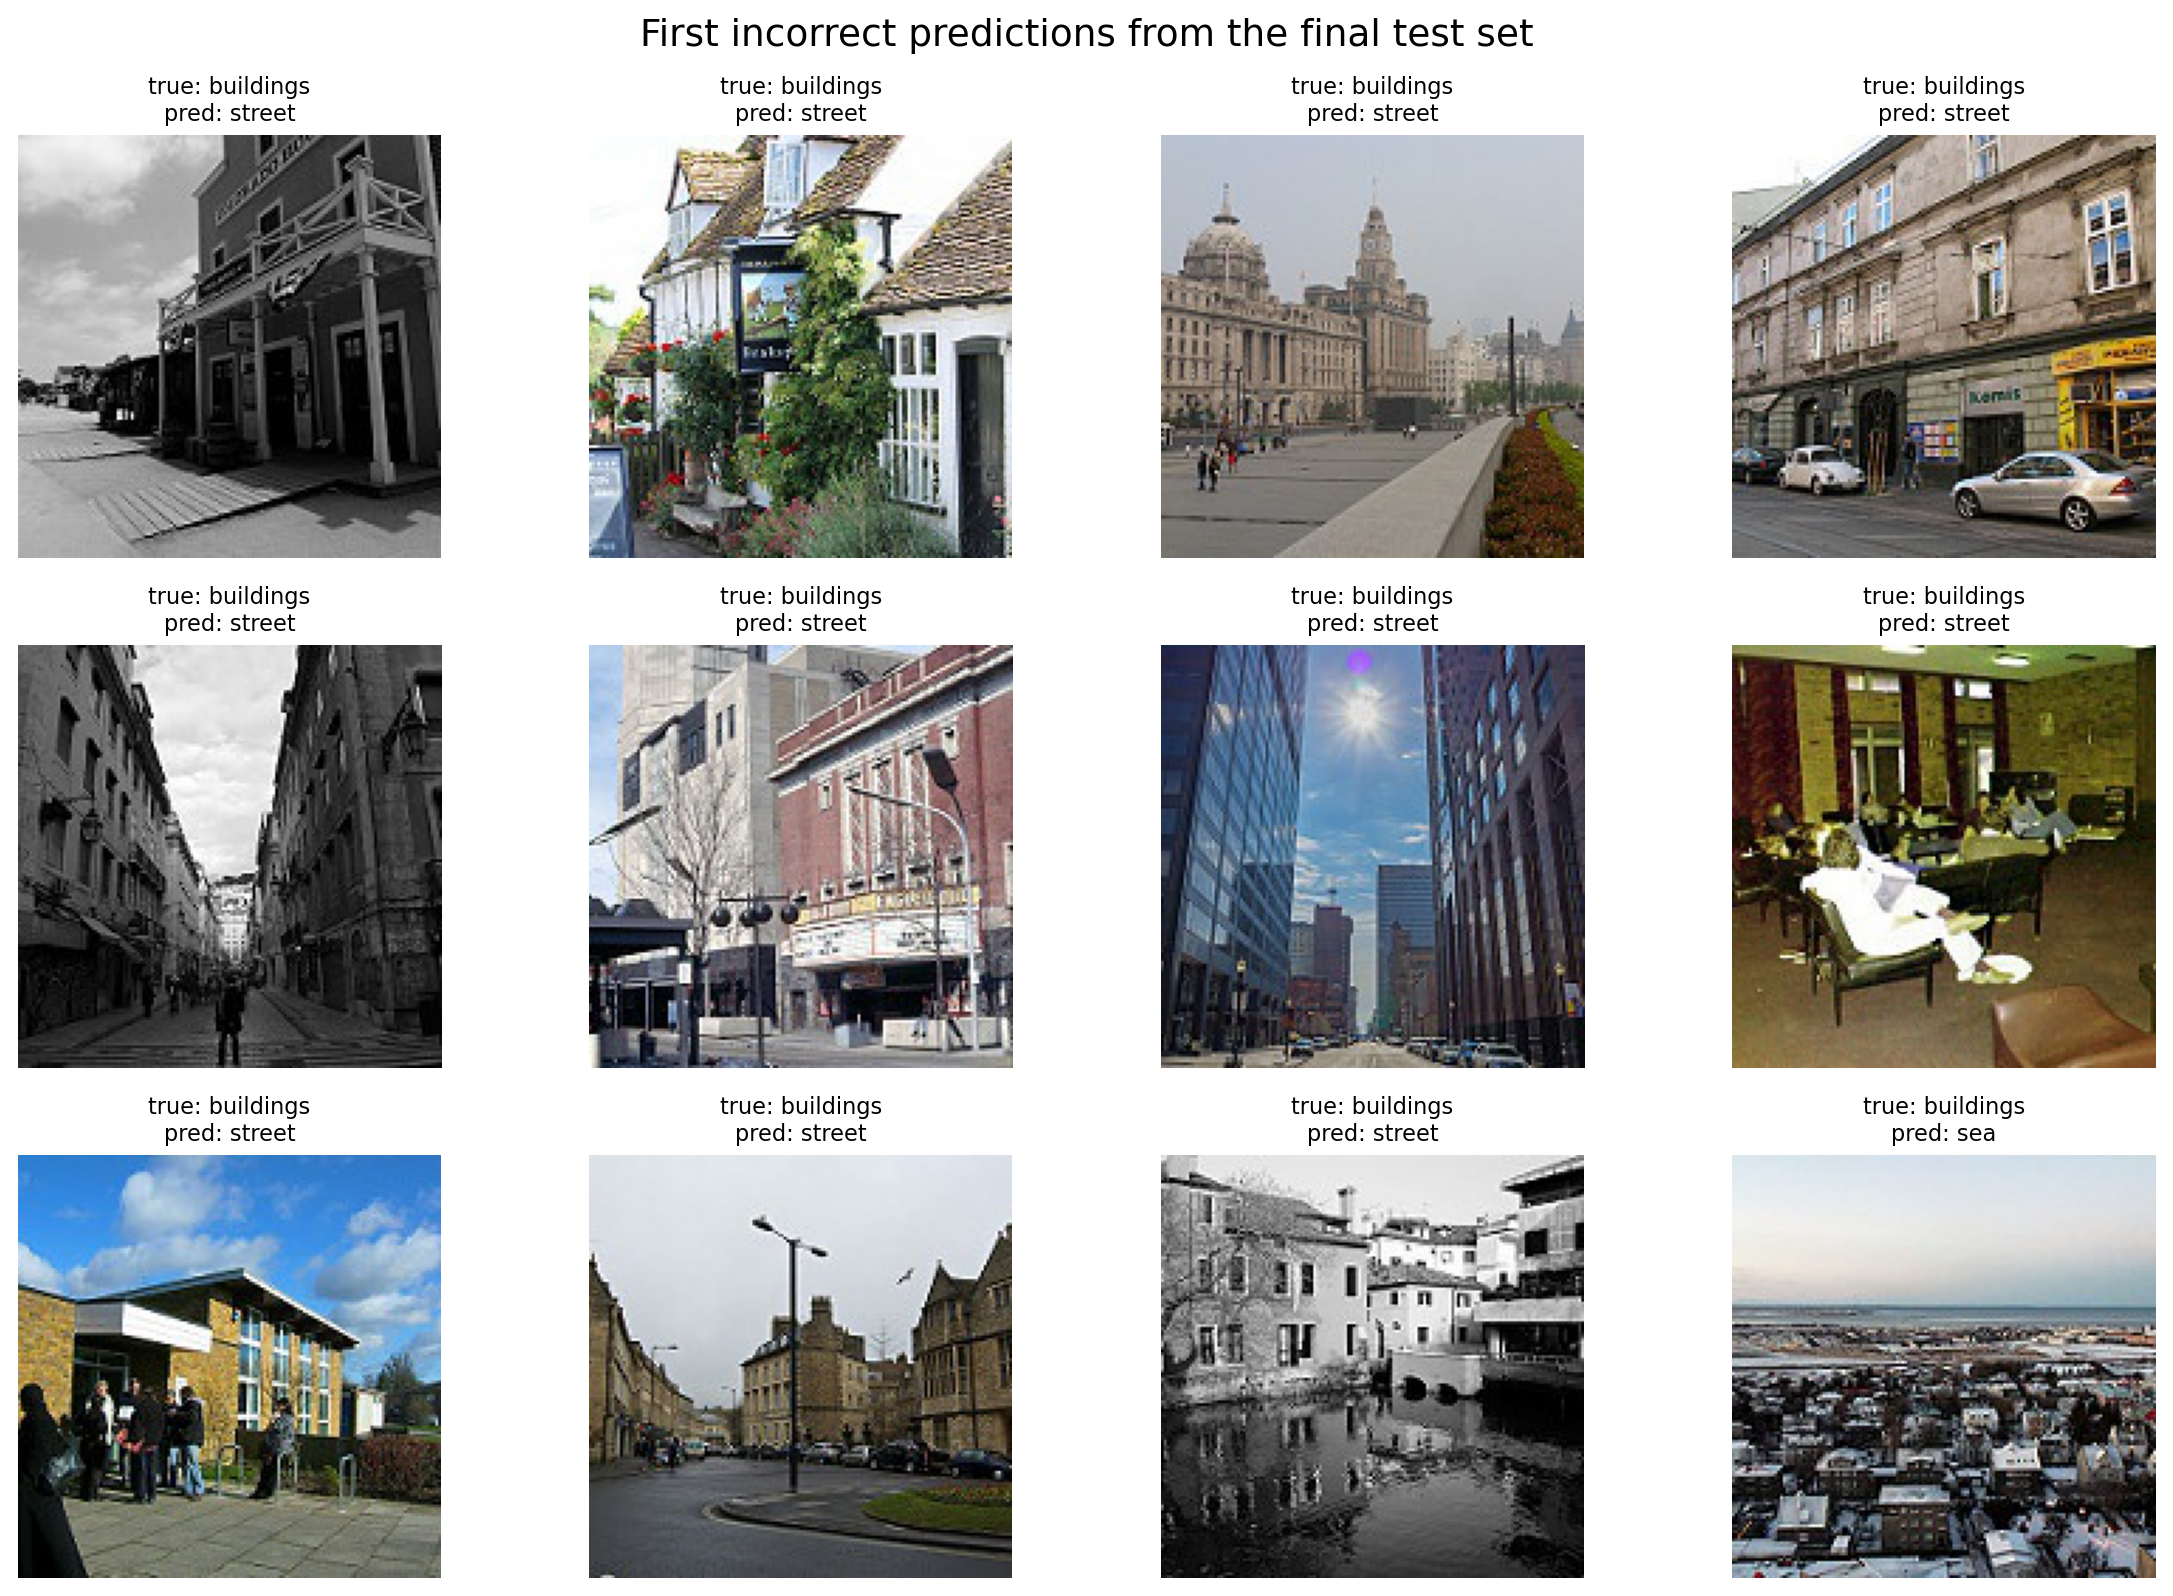
\includegraphics[width=\textwidth]{images/intel_08_error_examples.png}
\caption{Twelve incorrect predictions from the selected model on the untouched source test set.}
\label{fig:intel-errors}
\end{figure}

\begin{importantbox}
\textbf{Image conclusion.} Pretrained MobileNetV3-Small features plus balanced Logistic Regression are a strong, simple, and reproducible baseline for Intel scene classification. The result meets the assignment workflow because EDA, augmentation, a pretrained deep representation, a validation comparison, and a final untouched test evaluation are all present. It is still a classroom model: it can confuse visually related scenes and should not be treated as a general-purpose real-world scene understanding system.
\end{importantbox}
